\chapter{Grundlagen}

In den folgenden Abschnitten werden Grundlagen gelegt, welche für das weitere Verständnis der Studienarbeit benötigt werden.

\section{LEGO}

Hier steht nachher Zeugs, was mit Lego zu tun hat. Dazu gehört die WeDo-Kästen und auf jeden Fall der Wettbewerb, zumindest sollte definiert werden, warum die Kinder eigentlich mitmachen.

\section{Persönlichkeitscharaktere}

Der folgende Abschnitt geht genauer auf den Test für den Persönlichkeitstypus der einzelnen Kinder ein.

Der Test, den die Kinder durchgeführt haben, ordnet jedem Teilnehmer eine Tier zu. Jedes dieser Tiere steht für einen Typus nach dem \acrlong{mbti} (\acrshort{mbti}). Der \acrshort{mbti} besteht aus 16 verschiedenen Persönlichkeitstypen (vgl. Abbildung \ref{img:mbti}), bei denen jede der Typ die Überlagerung aus vier verschiedenen Attributen ist. Wie in der Abbildung dargestellt, gibt es damit 16 verschiedene Anordnungen der Zeichen E, F, I, J, N, P, S und T, wobei jedes Zeichen für ein bestimmtes Attribut steht. Insgesamt werden aus diesen Zeichen vier Paare gebildet: EI, SN, TF und JP. In einer Abkürzung nach Myer-Briggs kann jeweils nur ein Buchstabe eines Paares vorkommen, woraus die 16 Typen in Abbildung \ref{img:mbti} resultieren.
\begin{figure}[htbp!]
	\centering
	\fbox{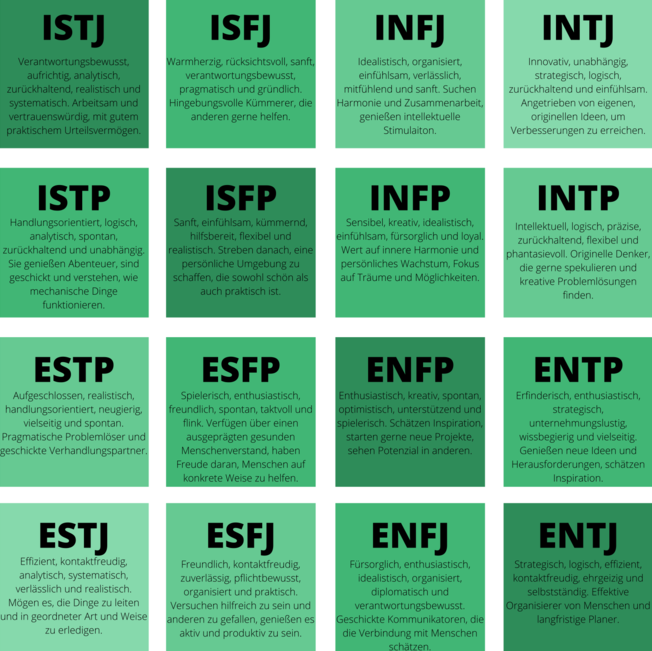
\includegraphics[width=0.35\textheight,angle=0]{img/Myers-Briggs-Typenindikator}}
	\caption[Myers-Briggs-Typenindikator]{Die 16 Persönlichkeitstypen nach Myers-Briggs}
	\label{img:mbti}
\end{figure}

Jeder einzelne Typ hat nach Myers-Briggs Auswirkungen auf Personen. \cite{myers_myers_2002} 
\lipsum[0-3]
\begin{figure}[htbp!]
	\centering
	\fbox{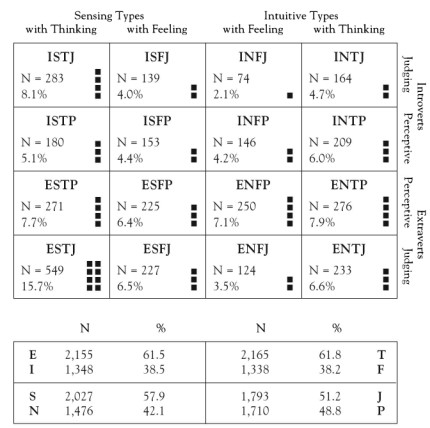
\includegraphics[width=0.35\textheight,angle=0]{img/distribution}}
	\caption[Verteilung der Myers-Briggs-Typen]{Verteilung der Myers-Briggs-Typen \cite{myers_myers_2002}}
	\label{img:mbti_distribution}
\end{figure}

\subsection{Studienrelevante Persönlichkeitscharaktere}
\subsubsection{Border Collie - ESTJ / ENTJ}
\begin{figure}[htbp!]
	\centering
	\fbox{
\includegraphics[width=0.2\textheight,angle=0]{img/Border_Collie}}
	\caption[Border Collie]{Border Collie}
	\label{img:Border_Collie}
\end{figure}
“Collie” is the Scottish Gaelic word for “useful.” They are logical, determined, competent and organized and prefer an environment where they can use their intelligence, lead others and are kept active. These kiddos are happiest when given opportunities to be in charge and compete. They enjoy challenges, debates and interacting with a variety of people. Life is one big competition, and they're determined to win. \\
\subsubsection{Elefant - ESFJ / ENFJ}
\begin{figure}[htbp!]
	\centering
	\fbox{
\includegraphics[width=0.2\textheight,angle=0]{img/Elephant}}
	\caption[Elefant]{Elefant \cite{knowAndLove}}
	\label{img:Elefant}
\end{figure}
Friendly, outgoing and organized. They're happiest when helping others, planning social events or participating in activities that involve people - ALL of the people. These kiddos prefer a harmonious and cooperative environment with lots of praise and affection. Life is all about genuine relationships and connecting with people.	\\
\subsubsection{Erdmännchen - INFP / ISFP}
\begin{figure}[htbp!]
	\centering
	\fbox{
\includegraphics[width=0.2\textheight,angle=0]{img/Meerkat}}
	\caption[Erdmännchen]{Erdmännchen \cite{knowAndLove}}
	\label{img:Elephant}
\end{figure}
Moralistic, gentle and sensitive with a creative yet complex inner world. They're happiest in calm, cooperative and supportive environments where they can pursue meaningful matters. These kiddos need plenty of scheduled alone time to process their natural gut feelings and analyze the world. They are deeply in tune with others' feelings and needs and tend to take on a peacemaker role. Life is about understanding what makes people tick. \\	
\subsubsection{Panda - INFJ / INTJ}
\begin{figure}[htbp!]
	\centering
	\fbox{
\includegraphics[width=0.2\textheight,angle=0]{img/Panda}}
	\caption[Panda]{Panda \cite{knowAndLove}}
	\label{img:Panda}
\end{figure}
	Intensely private, creative and idea-oriented. They're happiest when their efforts and unique ideas help others to grow and learn. They appreciate autonomy and being trustworthy, unique, capable and insightful individuals. These kiddos prefer a calm environment where they can think, process and create in their inner world. Understanding the meaning behind things is their goal in life. \\
\subsection{Restliche Tiere}
Im folgenden wird zur Einordnung der bereits genannten Tiere in das gesamte Spektrum der Persönlichkeitstypen mit den Tieren, welchem keinem Kind in der Studie zugeordnet wurde, dargestellt.



\section{Computational Thinking}

\section{Torrance Tests}{
	\label{sec:torrance_tests}
	\begin{figure}[htbp!]
		\centering
		\fbox{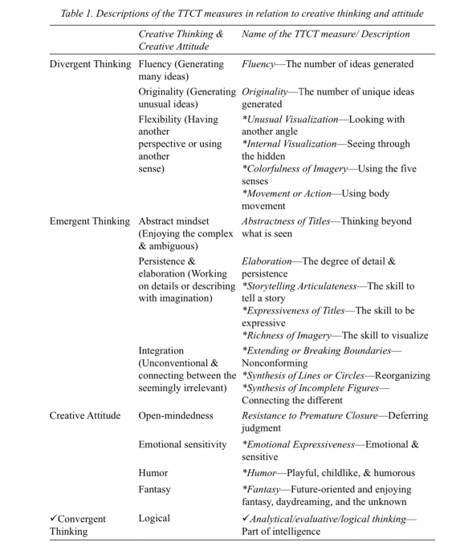
\includegraphics[width=0.4\textheight,angle=0]{img/ttct}}
		\caption[Relation von TCTT-Maßnahmen]{Relation von TCTT-Maßnahmen gegenüber kreativem Denken und kreativer Haltung \cite{Kim2016}}
		\label{img:ttct}
	\end{figure}
}
